\documentclass{article}
\usepackage{amsmath}
\usepackage{amssymb}
\usepackage{graphicx}
\begin{document}

\title{The Exponential and Gamma Distributions}
\author{Arthur Lui and Alexis Cottam}
\date{October 11, 2013}
\def\wl{\par \vspace{\baselineskip}}

\maketitle



\section*{Exponential Distribution}
\subsection*{Introduction}
The exponential distribution is a distribution used to model the time between events happening, such as poisson events.  The pdf of the exponential is based on the one parameter $\beta$, which is the average of what is being modeled.   


\subsection*{Derivations}

\subsubsection*{PDF}


$f(x \vert \beta) = \frac{1}{\beta}e^{(-x/\beta)},     0 \leq x < \infty,  \beta > 0$  \\
The parameter $\beta$ is a scale parameter.


%Integrates to 1
\begin{align*}
\int_0^\infty f(x) \mathrm{d}x &=  \int_0^\infty \frac{1}{\beta}e^{(-x/\beta)} \mathrm{d}x 
\\ &= - e^{(-x/\beta)} \bigg\vert_0^\infty \\ &= 0 - -1 \\ &= 1
\end{align*}

%Picture
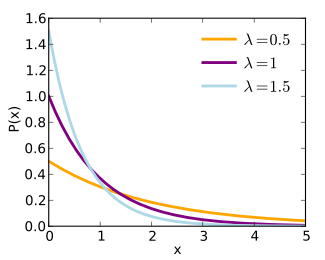
\includegraphics[scale=.50]{exppdf.png}
Note: $\lambda = \frac{1}{\beta}$ 
\subsubsection*{CDF}
$F(x) = 1 - e^{(-x/\beta)} , 0\leq x < \infty$
\begin{align*}
F(x) &= \int_0^x f(t) \mathrm{d}t \\
&=  \int_0^x  \frac{1}{\beta}e^{(-t/\beta)} \mathrm{d}t \\
&= - e^{(-t/\beta)} \bigg\vert_0^x \\
&= - e^{(-x/\beta)} - -1 \\
&= 1  - e^{(-x/\beta)}
\end{align*}

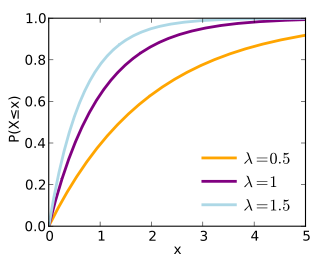
\includegraphics[scale=.50]{expcdf.png}
Note: $\lambda = \frac{1}{\beta}$ 
\footnote{Images of the exponential distribution pdf and cdf are from http://en.wikipedia.org/wiki/Exponential\_distribution.}


\subsubsection*{Mean and Variance}

$E(X) = \beta$

\begin{align*}
E(X) &=  \int_0^\infty \frac{x}{\beta}e^{(-x/\beta)} \mathrm{d}x \\
\textrm{Let}\:\: u=x   \:\:\:    \mathrm{d}v = e^{(-x/\beta)} \mathrm{d}x \\
 \mathrm{d}u =  \mathrm{d}x       \:\:\:        v= - \beta  e^{(-x/\beta)}\\ 
&= \frac{1}{\beta}\bigg[ -\beta x  e^{(-x/\beta)} \bigg\vert_0^\infty - \int_0^\infty -\beta  e^{(-x/\beta)} \mathrm{d}x\bigg] \\
&=  \frac{1}{\beta}\bigg[0 + \beta(- \beta e^{(-x/\beta)} \bigg\vert_0^\infty\bigg] \\
&=  \frac{1}{\beta}\bigg[0- - \beta^2\bigg] \\
&= \beta
\end{align*}\\


$Var(X) = \beta^2$
\begin{align*}
E(X^2) &=  \int_0^\infty \frac{x^2}{\beta}e^{(-x/\beta)} \mathrm{d}x \\
\textrm{Let}\:\: u=x^2   \:\:\:    \mathrm{d}v = e^{(-x/\beta)} \mathrm{d}x \\
 \mathrm{d}u =  2x\mathrm{d}x       \:\:\:        v= - \beta  e^{(-x/\beta)}\\ 
&= \frac{1}{\beta}\bigg[ -\beta x^2  e^{(-x/\beta)} \bigg\vert_0^\infty - \int_0^\infty -\beta  e^{(-x/\beta)} 2x\mathrm{d}x\bigg] \\
&=  \frac{1}{\beta}\bigg[0 + \int_0^\infty 2x \beta e^{(-x/\beta)}\mathrm{d}x\bigg] \\
&=   \int_0^\infty 2x e^{(-x/\beta)}\mathrm{d}x \\
\textrm{Let}\:\: u=2x   \:\:\:    \mathrm{d}v = e^{(-x/\beta)} \mathrm{d}x \\
 \mathrm{d}u =  2\mathrm{d}x       \:\:\:        v= - \beta  e^{(-x/\beta)}\\ 
&= -2x\beta e^{(-x/\beta)}\bigg\vert_0^\infty - \int_0^\infty -2 \beta  e^{(-x/\beta)} \mathrm{d}x \\
&= 0 - 2 \beta^2  e^{(-x/\beta)} \bigg\vert_0^\infty \\
&= 0 - - 2 \beta^2 \\
&=2\beta^2 
\end{align*}\\

\begin{align*}
Var(X) &= E(X^2) - [E(X)]^2\\
&=2\beta^2 - \beta^2\\
&=\beta^2
\end{align*}

\subsubsection*{Moment Generating Function}

$M_{x}(t) = \frac{1}{1-\beta t} , t<\frac{1}{\beta}$

\begin{align*}
M_{x}(t) &= E(e^{tx})\\
&= \int_0^\infty \frac{e^{tx}}{\beta}e^{(-x/\beta)} \mathrm{d}x \\
&=  \frac{1}{\beta} \int_0^\infty e^{x(t-\frac{1}{\beta})} \mathrm{d}x\\
&= \frac{1}{\beta}\bigg[ \frac{ e^{x(t-\frac{1}{\beta})}}{t-\frac{1}{\beta}}\bigg\vert_0^\infty \bigg]\\
&=  \frac{1}{\beta}\bigg[0 - \frac{1}{t-\frac{1}{\beta}}\bigg] \:\:\:\textrm{where}\:\:\: t < \frac{1}{\beta}\\
&= \frac{-1}{\beta t - 1} \\
&= \frac{1}{1-\beta t}
\end{align*}


\subsection*{Uses of the Distribution}

\subsubsection*{Relation to Other Distributions}
The Exponential distribution is related to the Uniform, Gamma and Weibull distributions.
\\
If $X\sim Uniform$ and $Y=-log(X)$, then $Y\sim Exp$.
\\
If $X\sim Gamma(\alpha = 1, \beta)$, then $X\sim Exp(\beta)$.
\\
If $X\sim Exp$ and $Y=X^{(1/\gamma)}$, then $Y\sim Weibull$. 
\\
\\Also, the exponential distribution is the continuous form of the geometric distribution.  Where the geometric distribution can model time between events in the discrete case, the exponential can model these times in the continuous case.
\subsubsection*{Example}
If the average waiting time at a doctor's office is $\beta = 20$ minutes, what is the probability that you will have to wait less than 10 minutes?
\\
$P(X \leq 10) = \int_0^{10} f(x)\mathrm{d}x = 0.3934693$
\\
\\The exponential distribution is a good model for waiting times, lifetimes, and decay because these tend to follow exponential distributions.  When an average rate of occurance is known and the rate is believed to be exponentially distributed, the exponential distribution is a good choice as a model.    


\subsubsection*{Other Uses for the Distribution}
 
The exponential distribution is also used to model time between Poisson events.   
\\
\\
An interesting characteristic is that the exponential distribution is memoryless.
\\
$P( X > s | X> t) = P(X > s-t)$
\\
For example: Given you have waited 20 minutes, the probability you'll wait 30 minutes is the same as the probability you'll wait 10 minutes. 
 





\section*{Introduction:}

  \subsection*{The Gamma Function:}
    The Gamma Function is defined as:
    \[
      \Gamma (\alpha) = \int\limits_0^\infty {t^{\alpha - 1} e^{-t} dt},
    \]
    where $\alpha > 0$.\\\\
   \subsection*{ Useful Identities:}
    \[
      \Gamma(\alpha+1) = \alpha\Gamma(\alpha), ~~~\alpha > 0
    \]
    \[
      \Gamma(n) = (n-1)!, ~~~ n ~ \epsilon ~ \mathbb{N}
    \]
    \[
      \Gamma(1) = 1
    \]
    \[
      \Gamma(\frac{1}{2}) = \sqrt(\pi)
    \]
  \subsection*{Derivation of the Gamma Distribution:}
     Consider
     \[
        f(t) = \frac{t^{\alpha-1} e^{-t}}{\Gamma(\alpha)},~~0~<~t~<\infty.
     \] 
     Integrating f(t) from $0~to~\infty$, we get
     \[
        \int\limits_0^\infty {f(t) dt} = 
        \int\limits_0^\infty {\frac{t^{\alpha - 1} e^{-t}}{\Gamma(\alpha)} dt} =
        \frac{\int\limits_0^\infty {t^{\alpha - 1} e^{-t}} dt}{\Gamma(\alpha)}
     \]
     \[
        = \frac{\Gamma(\alpha)}{\Gamma(\alpha)}
     \]
     \begin{equation} 
        = 1.
     \end{equation}
     Therefore, f(t) is a pdf. 

\section*{Derivation:}

  \subsection*{pdf:}
  Let $X \sim \beta T $ in (1), where $\beta > 0$. Then the $ gamma(\alpha,\beta) $ family is defined below as:
  \[
    f(x|\alpha,\beta) = \frac{1}{\Gamma(\alpha)\beta^\alpha}x^{\alpha-1}e^{-x/\beta}, ~~~ 0<x<\infty,~~~\alpha>0,~~~\beta>0.
  \]
  The parameters $\alpha$ and $\beta$ are referred to as the shape and scale parameters respectively as the $\alpha$ most influences the peakedness of the distribution, while $\beta$ most influenxes the spread of the distribution.

  \begin{center}
  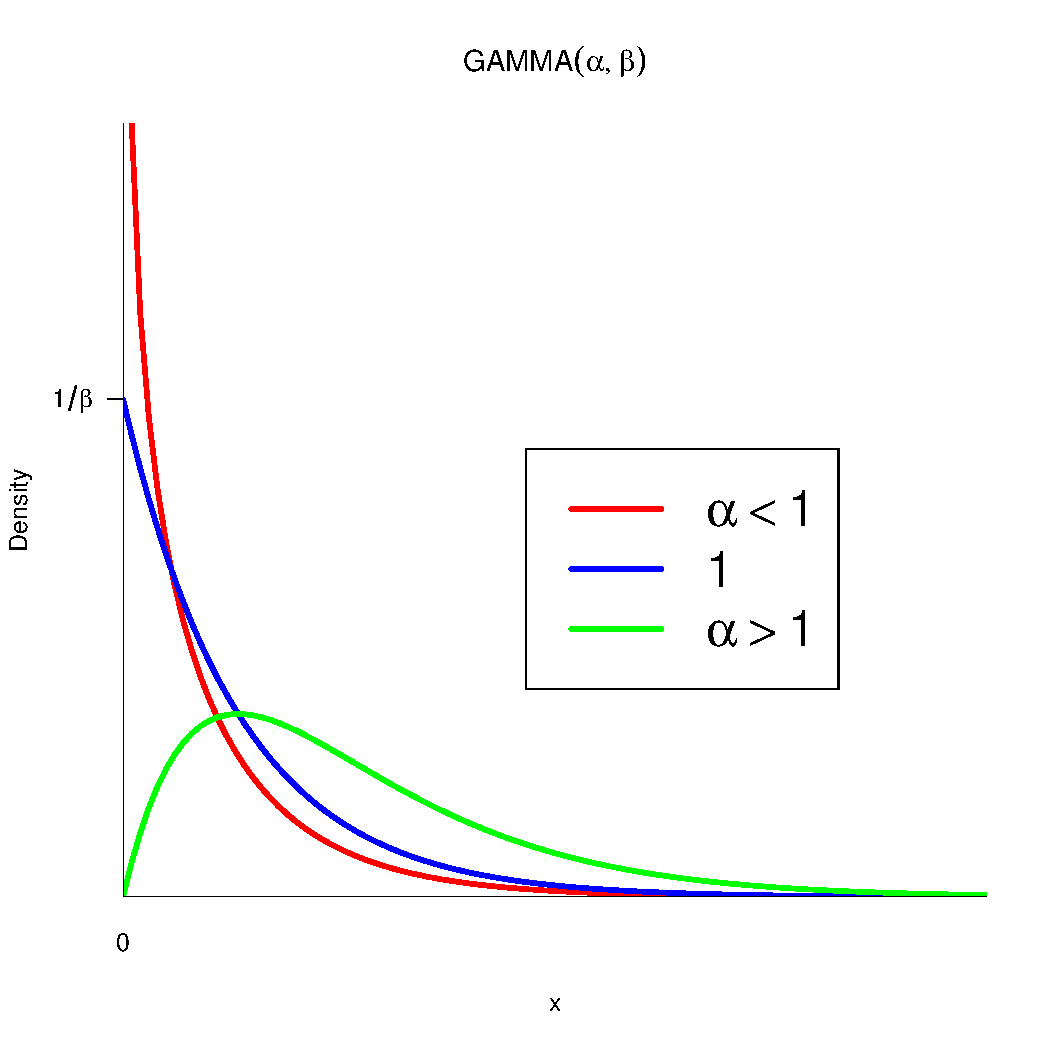
\includegraphics[scale=.5]{plot.pdf}
  \end{center}

  \subsection*{Integration to 1:}
  Let $X \sim \Gamma(\alpha,\beta)$, $x,\alpha,\beta > 0$. Then,
  \[
    \int\limits_0^\infty {f(x)dx}
  \]
  \[
    = \int\limits_0^\infty {\frac{1}{\Gamma(\alpha)\beta^\alpha}x^{\alpha-1}e^{-x/\beta}dx}
  \]
  \[
    = \frac{1}{\Gamma(\alpha) \beta^\alpha} \int\limits_0^\infty{x^{\alpha-1}e^{-x/\beta}dt}
  \]
  \[
    = \frac{\beta\beta^{\alpha-1}}{\Gamma(\alpha)\beta^\alpha} 
      \int\limits_0^\infty {\frac{x^{\alpha-1}}{\beta^{\alpha-1}}e^{-x/\beta}d\frac{x}{\beta}}
  \]
  \[
    = \frac{\beta^{\alpha}}{\Gamma(\alpha)\beta^\alpha}
      \int\limits_0^\infty
    { \left(\frac{x}{\beta}\right) ^ {\alpha-1} e^{-\frac{x}{\beta}} d\frac{x}{\beta}}
  \]
  \[
    = \frac{1}{\Gamma(\alpha)} \int\limits_0^\infty {t ^ {\alpha-1} e^{-t} dt}
  \]
  \[
    \frac{1}{\Gamma(\alpha)} \Gamma(\alpha) = 1.
  \]
  Therefore, f(x) integrates to 1. 
 
  \subsection*{CDF}
  The Gamma Cumulative Distribution is function is given by:
  \[
    \frac{\gamma(k,x/\theta)}{\Gamma(k)},
  \]
  where $k > 0$, and
  \[ 
    \gamma(k,x/\theta) = \int\limits_0^{x/\theta} {t^{k-1}e^{-t}dt}
  \]
  \section*{Mean and Variance:}
  \[
    E[X] = \alpha \beta 
  \]
  \subsection*{Proof:}
  \[
    E[X] = \int\limits_0^\infty {x\frac{1}{\Gamma(\alpha)\beta^\alpha}
                                 x^{\alpha-1} e^{-x/\beta} dx}
  \]
  \[
    = \frac{\Gamma(\alpha+1)\beta^{\alpha+1}}{\Gamma(\alpha)\beta^\alpha} 
      \int\limits_0^\infty {
        \frac{1}{\Gamma(\alpha+1)\beta^{\alpha+1}} 
        x^{\alpha+1} e^{-x/\beta}
      dt}
  \]
  \[
    = \frac{\Gamma(\alpha+1)\beta^{\alpha+1}}{\Gamma(\alpha)\beta^\alpha}
  \]
  \[
    = \frac{\Gamma(\alpha+1)}{\Gamma(\alpha)}\beta
  \]
  \[
    = \frac{\alpha\Gamma(\alpha)}{\Gamma(\alpha)}\beta
  \]
  \[
    = \alpha\beta
  \]
  \wl
  \[
    Var[X] = \alpha \beta^2
  \]
  \subsection*{Proof:}
  \[
    E[X^2] = \int\limits_0^\infty {x^2\frac{1}{\Gamma(\alpha)\beta^\alpha}
                                 x^{\alpha-1} e^{-x/\beta} dx}
  \]
  \[
    = \frac{1}{\Gamma(\alpha)\beta^{\alpha}} 
      \int\limits_0^\infty { x^{(\alpha+2)-1} e^{-x/\beta}dx}
  \]
  \[
    \frac{\Gamma(\alpha+2)\beta^{\alpha+2}}{\Gamma(\alpha)\beta^{\alpha}}
  \]
  \[
    = (\alpha+1)\alpha\beta^2
  \]
  \wl
  Therefore,
  \[
    Var[X] = E[X^2] - (E[X])^2
  \]
  \[
    =(\alpha+1)\alpha\beta^2 - (\alpha\beta)^2
  \]
  \[
    = \alpha\beta^2
  \]
  \section*{Moment Generating Function:}
  \[
    M_x(t) = E[e^{tx}] = {\left( \frac{1}{1-\beta^t} \right)} ^ \alpha
  \]
  \[
    M_x(t) = \int\limits_0^\infty { e^{tx} \frac{1}{\Gamma(\alpha)\beta^\alpha} 
                                    e^{-x/\beta} x^{\alpha-1}dx}
  \]
  \[
    = \int\limits_0^\infty { \frac{1}{\Gamma(\alpha)\beta^\alpha} 
                             e^{-(x/\beta) + tx}x^{\alpha-1}dx}
  \]
  \[
    = \frac{1}{\beta^\alpha} \int\limits_0^\infty { 
      \frac{ \left( {\frac{1}{(1/\beta)-t}} \right)^\alpha } 
            {\left( \Gamma(\alpha){\frac{1}{(1/\beta)-t}} \right) ^\alpha}
      e^{-x/\frac{1}{(1/\beta)-t} } x ^ {\alpha-1} dx}
  \]
  \[
    = \left( {\frac{1}{(1/\beta)-t}} \right)^\alpha / \beta^\alpha
  \]
  \[
    = \left( {\frac{1}{[(1/\beta)-t]\beta}} \right)^\alpha
  \]
  \[
    = \left( \frac{1}{1-\beta t}\right) ^ \alpha
  \]

  \subsection*{Relation to Other Distributions:}
  \textbf{Poisson-Gamma.} The Gamma distribution is a conjugate prior
  for the mean of the Poisson distribution.\\
  \textbf{Exponential-Inverse Gamma.} The Inverse Gamma distribution is a
  conjugate prior for the mean of the exponential distribution. \\
  \wl
  \textbf{Exponential.} $Gamma(1,\beta) = EXP(\beta)$.\\
  \textbf{Chi-Sqaured.} $Gamma(p/2,2) = \chi ^2 (p)$.\\
  \textbf{Maxwell.} Let X be distributed as a Gamma. If $\alpha = 3/2$, then $Y = \sqrt{X/\beta}$ is distributed as a Maxwell.\\
  \textbf{Inverse Gamma.} Let $X \sim Gamma(\alpha,\beta)$. Then $Y = 1/X \sim InverseGamma(\alpha,\beta)$.\\
  \wl
  \textbf{More on Poisson-Gamma.} The Negative Binomial can be derived as a gamma mixture of Poissons.\\
  \wl
  Specifically, if
  \[
     X \sim NB (r,\beta)
  \]
  and
  \[
    X|\lambda \sim POI(\lambda),
  \]
  then
  \[
    \lambda \sim Gamma(r,\beta).
  \]


  \subsection*{Applications of the Gamma Distribution:}
  The Gamma distribution is positive and right-skewed, so it is can be used to model a variety of events, including the following:
    \wl
    \wl
    - The amount of rainfall accumulated in a reservoir\\
    - The size of loan defaults of aggregate insurance claims\\
    - The flow of items through manufacturing and distribution processes\\
    - The load on web servers\\
    - The many and varied forms of telecom exchange

  \subsection*{Example:}
  Suppose that for a graduate Statistical Computing course, the average time required for every student to come up with a feasible solution for each exam problem is two hours. Compute the probability that a student, say Mickey, will take 8 or more hours to come up with the solutions to all four problems of the exam.\\
\wl
One problem every 2 hours means we would expect to "solve" $\beta = 1/2$ exam problems every hour on average. Using $\beta = 1/2 $ and $\alpha = 16$, we can compute this as follows:
\[
  P(X \ge 8) = \int\limits_8^\infty {\frac{x^{16-1}e^{-x/.5}}{\Gamma(16)(1/2)^{16} }dx}
             = .466745
\]


\end{document}


